\section{简介}

如图~\ref{fig:overview},以C++为基本,对基础部分进行学习。
了解C++基本语法,学习类与数据对象,容器和算法,\textbf{面向对象和泛型编程(重点)},编译与底层,C++新特性。

\begin{figure}[]
	\centering
	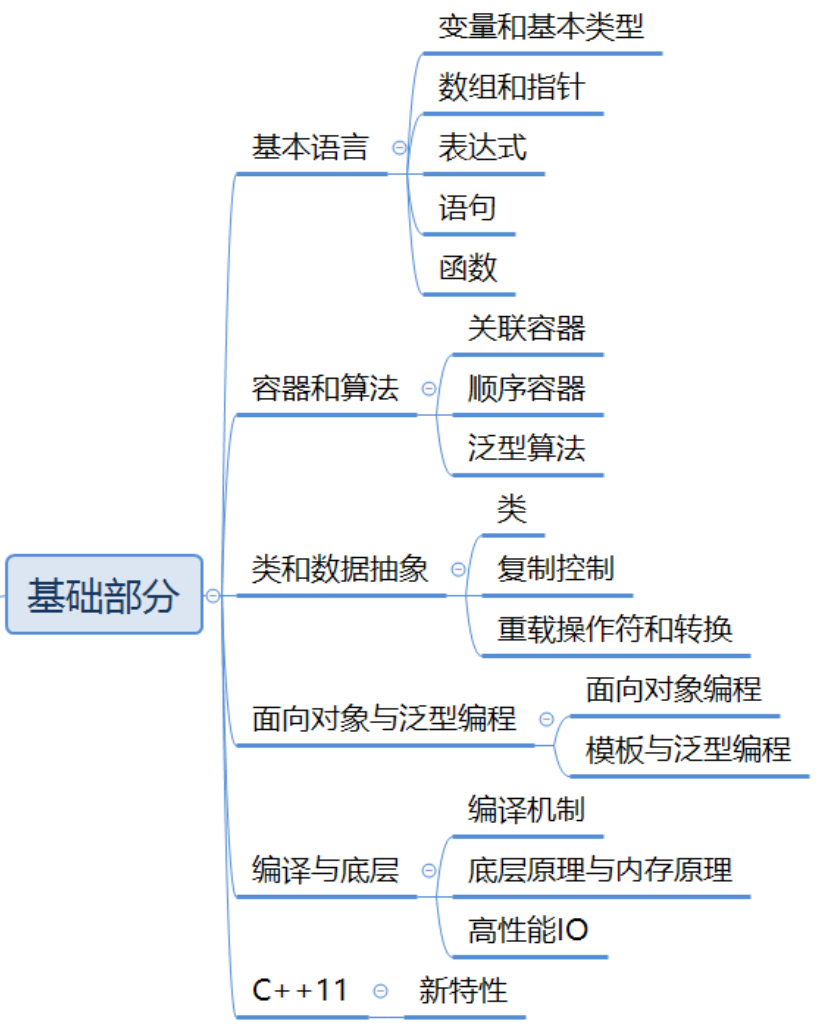
\includegraphics[width=0.5\columnwidth]{pic/overview.png}
	\caption{基础部分学习总览}
	\label{fig:overview}
	% \vspace{-5pt}
\end{figure}

\section{开始}
C++语言同时支持五种编程风格:C风格(面向过程)、基于对象、面向对象、泛型和函数式。
在C++11之前抽象存在若干的缺陷,最严重的是缺少自动内存管理和对象级别的消息发送机制。
现代C++语言可以看作是三部分组成的:1.低级语言,大部分继承自C;2.现代高级语言特性,允许我们定义自己的类型以及组织大规模程序和系统;3.标准库,利用高级特性来提供有用的数据结构和算法。
\begin{tcolorbox}[boxsep=-0.05in]
	\underline{C++和C有什么区别:} C++有与C一样的低级语言特性,面向过程,这部分主要继承于C;同时C++,尤其是C++11拥有众多的高级语言特性,使得程序更加易于开发,提供非常多的标准库,使得实现特定的数据结构和算法更加简单。同时,C++相比于C,它支持更多的编程模式,比如面向对象,基于对象,函数式编程以及泛型编程。
	\textbf{参考答案:}设计思想上,C++是面向对象的语言,而C是面向过程的结构化编程语言;语法上,C++具有封装、继承和多态三种特性,C++相比C,增加多许多类型安全的功能,比如强制类型转换、C++支持范式编程,比如模板类、函数模板等。
\end{tcolorbox}

\subsection{关键字总结}
\begin{itemize}
	\item \textbf{基本内置类型:} 算术类型(整形(包括字符和布尔)|浮点型):bool, char, wchar\_r, char16\_t, char32\_t, short, int, long, long long, float, double, long double。 bit(1)-byte(8)-word(32/64) byte是寻址的最小内存单元。无符号数永远不会小于零,切勿混用。'a'单引号是char型字面值,"hello"叫字符串字面值,字符串型字面值结尾会补一个空字符。
	\item \textbf{初始化和赋值}要加以区分,但事实上无关紧要。赋值是将对象的当前值擦除,而以新值代替。建议初始化所有的内置类型的变量。
	\begin{lstlisting}[caption={}]
		int units = 0;
		int units = {0};
		在C++11中用花括号初始化变量得到了全面的应用,该形式称为列表初始化。该方式在赋值中如何会丢失值(非强制类型转换),编译器会报错。
		int units{0}; 
		int units(0);
	\end{lstlisting}
	\item \textbf{extern} 为了支持分离式编译,C++将声明和定义区分开来。声明只是让名字为程序所知,而定义负责创建与名字关联的实体。在实际执行上,定义申请存储空间,也可能会赋初值,而声明不会。 extern int i; int j; 但是extern int i = 1;是声明,因为包含了显示初始化。变量能且只能被定义一次,但是可以被多次声明。主要用来解决多个文件中使用同一个变量的情况。
	\item \textbf{复合类型}指基于其他类型定义的类型,如引用和指针。一般情况下说引用就是指左值引用,而在C++11中新增了右值引用。
	\item \textbf{引用} int ival = 1024; int $\&$ref = ival;引用必须被初始化。引用即别名,相当于又起了一个名字。
	
	
	
	\item \textbf{输入输出流:} iostream,$cin >>$, $cout <<$。
	\item \textbf{控制流:} while(condition) {statement} ; for(int i=1;i<=10;++i){statement} ; if(condition){statement};
	\item \textbf{类:} 一个类型,以及与其关联的一组操作。同.来访问成员。
	\begin{lstlisting}[caption={}]
		
		
		sales_item item;
	\end{lstlisting}
	
	
	
	  
	\item \textbf{static}关键字:在全局变量前面的时候,定义一个全局静态变量,在静态存储区,整个程序运行期间一直存在,未被初始化的全局静态变量将自动初始化为0,作用域在声明他的文件之外不可见。相对应的,局部静态变量,大体与全局静态变量是一样的,只是作用域只停留在局部,当方法退出时,全局静态变量不销毁而是继续驻留在静态存储区,直到方法被再次调用。
\end{itemize}
